\documentclass{ieeeaccess}

% Custom packages
\usepackage{caption}
\usepackage{subcaption}
\usepackage{hyperref}
\hypersetup{breaklinks=true}
\usepackage[nolist, printonlyused]{acronym}
\usepackage{enumerate}


% Template packages
\usepackage{cite}
\usepackage{amsmath,amssymb,amsfonts}
\usepackage{algorithmic}
\usepackage{graphicx}
\usepackage{textcomp}

\def\BibTeX{{\rm B\kern-.05em{\sc i\kern-.025em b}\kern-.08em
    T\kern-.1667em\lower.7ex\hbox{E}\kern-.125emX}}

\begin{document}
    \begin{acronym}
    \acro{REG}[REG]{renewable energy generator}
    \acro{ESS}[ESS]{energy storage system}
    \acro{BESS}[BESS]{battery energy storage system}
    \acro{PV}[PV]{photovoltaic}
    \acro{EMS}[EMS]{energy management system}
    \acro{DER}[DER]{distributed energy resource}
    \acro{EOL}[EOL]{end of life}
    \acro{SOC}[SoC]{state of charge}
    \acro{SOH}[SoH]{state of health}
    \acro{DOD}[DoD]{depth of discharge}
    \acro{BMS}[BMS]{battery management system}
    \acro{RUL}[RUL]{remaining useful life}
    \acro{EM}[EM]{electrochemical model}
    \acro{ECM}[ECM]{equivalent circuit model}
    \acro{MILP}[MILP]{mixed integer linear programming}

    \acro{LIB}[LIB]{lithium-ion battery}
    \acroplural{LIB}[LIBs]{lithium-ion batteries}

    \acro{MG}[MG]{microgrid}
    \acroindefinite{MG}{a}{an}
\end{acronym}

    \history{Date of publication xxxx 00, 0000, date of current version xxxx 00, 0000.}
    \doi{10.1109/ACCESS.2017.DOI}

    \title{A Novel Battery Wear Model For Energy Management In Microgrids}

    \author{
    	\uppercase{Marcos Aurelio Izumida Martins}\authorrefmark{1}
    	\uppercase{Lucas B. Rhode}\authorrefmark{2},
    	\uppercase{and Adriano B. de Almeida}\authorrefmark{3}
    }

    \address[1]{Sustainable Energies Center, CERTI Foundation, Brazil (e-mail: mlz@certi.org.br)}
    \address[2]{Underwriters Laboratories, Brazil (e-mail: lucas.rhode@ul.com)}
    \address[3]{Western Parana State University, Brazil (e-mail: adriano.almeida@unioeste.br)}

    \markboth
    {Author \headeretal: Preparation of Papers for IEEE TRANSACTIONS and JOURNALS}
    {Author \headeretal: Preparation of Papers for IEEE TRANSACTIONS and JOURNALS}

    \corresp{Corresponding author: Marcos A. I. Martins (e-mail: mlz@certi.org.br)}

    \begin{abstract}
        This paper proposes a novel battery wear model for \ac{MG} energy management applications. This model is based on a popular battery wear model originally proposed for vehicle-to-grid (V2G) applications. The presented model can be easily parameterized to fit the cycle life data of almost any battery and yields the wear cost of a charge/discharge event as function of the variation in the \ac{SOC} of the battery. This wear model is incorporated into an energy management algorithm to optimize the operation of a grid-connected \ac{MG} using a day-ahead planning strategy. To test the model, four simulated scenarios are considered in \iac{MG} composed of a \ac{DG}, a \ac{PV} system, a residential load and, naturally, a battery storage system (\ac{BESS}). The inclusion of the battery wear model leads the optimizer to be more selective about battery usage, cycling the battery at \ac{SOC} levels that minimized battery wear, effectively prolonging its lifespan.
    \end{abstract}

    \begin{keywords}
        battery management systems, energy storage, energy management, microgrids
    \end{keywords}

    \titlepgskip=-15pt

    \maketitle

    \section{Introduction}
    \label{sec:introduction}
    \PARstart{E}{lectricity} has become an essential element for society in the last century. With growing energy consumption aggravating the rise in CO\textsubscript{2} emissions, achieving full sustainability is one of the greatest challenges of our modern society. As part of this effort, grid operators are continually deploying new \acp{REG}, such as wind farms and \ac{PV} power stations, sources that supplied a record high of more than 11\% of the world's electricity in 2020 \cite{EMBER2021}.

    In \acp{MG}, \acp{REG} play a vital role and, as such, \acp{ESS} are one of the main components in these environments. While traditional generators can store energy in fuel tanks, water reservoirs and kinetic energy, most renewable sources need external devices to store their output when it is abundant to later return it to the grid \cite{STECCA2020}. Additionally, by combining renewable generation and energy storage, \ac{MG} operators can coordinate resources to achieve increased system efficiency by reducing generation-demand mismatches, using techniques such as time-shifting, peak shaving and valley filling \cite{WANG20196201, LI2020106058, PARRA2015576, ZHANG2019772}.

    There are many different technologies for storing energy, such as pumped hydros, fuel cells, flywheels, supercapacitors and others \cite{IBRAHIM2008}. However, \acp{BESS} are commonly the preferred choice for energy management applications. They present good energy density, scalability, efficiency and technical maturity, which makes them a good fit for energy storage in small-scale systems \cite{KOCER2019, martins2018optimal, FU20136749070}.

    Among the available technologies, \acp{LIB} and lead-acid are predominant in modern \ac{BESS} applications \cite{FU20136749070, ALSAIDAN8094981}. Historically, lead-acid batteries were preferred for their lower upfront cost, in spite of lithium cells having a greater overall performance and longevity \cite{wang2013li, xu2010lithium}. Recently, the growing interest in electric vehicles and the associated mass production have significantly reduced the cost of this technology, making it the most popular energy storage method in \acp{MG} \cite{mongird20202020, BBERG2020, zhang2018energy}.

    Still, \acp{BESS} are costly, which becomes even more evident when its useful lifespan is taken into account. Batteries have a limited number of achievable discharge and recharge cycles before they reach their \ac{EOL}, at which point the cells no longer meet minimal criteria for power system applications \cite{ZHU2021100537, hart2014modeling}.

    Usually the \ac{EOL} is defined as a reduction of 20\% to 30\% of the battery's \ac{SOH} in general applications \cite{ECKER2014, NARAYAN2018}. In more sensitive environments where performance of the \ac{ESS} is crucial, more specific criteria may apply \cite{WOOD20115147, JACOB2020101565}. To determine the \ac{SOH}, \acp{BMS} employ various methods and, although there is no fixed definition for \ac{SOH}, many references utilize the effective capacity to evaluate it and estimate the \ac{RUL} of a battery \cite{TIAN2020120813, rezvanizaniani2014review, BIOLOGIC2021, bose2002battery}.

    Since \ac{SOH} is an indicator of battery wear, each time a battery is charged or discharged it inevitably decreases. As such, the amount it varies at each cycle can be modeled as a function of operational conditions (e.g. \ac{SOC}, current and temperature) and correlated to the acquisition cost of the \ac{BESS} unit to be plugged into an optimizer and minimized.

    However, estimating the \ac{SOH} of a battery is challenging. Estimation models can be divided into experiment-based and model-based. Experimental models are attractive for being simpler in terms of computational complexity, however it requires a large number of experiments to assess how the variables change as cells age \cite{XIONG2018264}.

    In \cite{li2019lithium,kang2014new} machine learning and Big Data are modern approaches used to estimate the state of \ac{EV} batteries from voltage, current and temperature. The studies provide two \ac{LIB} models based on deep learning that are able to predict battery performance at different aging levels, both of which could be used to estimate \ac{SOH} and \ac{RUL}.

    Albeit these approaches can be very useful and present low error margins, literature still lacks the necessary data volume and diversity to correctly train a single model that can be easily transposed  to different batteries with varying composition, capacity and manufacturing processes \cite{maheshwari2020optimizing}.

    In fact, the acquisition of experimental data for each specific \ac{BESS} can be unrealistic in most practical cases, such as large scale projects that seek to implant many \acp{MG} for multiple different clients in various locations. Usually the \ac{MG} operator does not have the time, technical or financial resources to execute extensive tests. To overcome this, model-based methods can be applied.

    Model-based methods can be further categorized into \acp{ECM}, \acp{EM} or black box models. \Iac{ECM} can present a highly adaptive approach to achieve particularly accurate wear estimation. In \cite{XIONG2018264}, researchers are able to predict battery performance throughout its entire lifespan with remarkable accuracy, aided by a set of interdependent partial differential equations. The equations describe the reactions that occur in the anode, cathode and separator layer, however the inputs are complex to acquire, which can be detrimental in \ac{EMS} applications, which usually require lightweight solutions.

    In such cenarios, \iac{ECM} can offer a practical way to model both the static and dynamic behavior of cells for battery management in local controllers. This approach is useful since it can be parameterized and implemented to estimate multiple indicators such as \ac{SOC}, \ac{SOH} and power capability, as done in studies \cite{verbrugge2004adaptive, verbrugge2007adaptive}. However, it still demand a great knowledge of battery parameters, their interdependence and external conditions, such as temperature and operational history \cite{zhang2018online}.

    These approaches can certainly be made highly accurate with increased model complexity and data availability. However, in a centralized \acp{EMS} responsible for managing multiple microgrids across various locations the communication and hardware requirements for acquiring and processing all the necessary data can limit the applicability of these models \cite{DIMEASHATZIARGYRIOU2005}.

    In light of this, this paper seeks to provide a lightweight semi-empirical model in which the precision can be adjusted according to available processing power. More specifically, it proposes a novel aging model that blends both model and experiment-based approaches that require only simple \ac{ACC} curves that can be obtained relatively easily from datasheets or manufacturers and resellers. The goal of this formulation is to provide a simple wear cost quantifier that can be used to orientate the \ac{EMS} of \iac{MG} as to whether or not use the \ac{BESS} in detriment of other strategies -- such as dispatching \ac{DG}s or purchasing power from the utility grid -- rather then providing a highly accurate battery state predictor.

    We base our modified wear cost model on \cite{HAN2014} and add to the state of the art:
	\begin{enumerate}[i]
    	\item a generic wear cost quantification, which operators can easily fine-tune to their own scenarios;
    	\item a concrete implementation of that formulation that can be parameterized to fit lead-acid and \ac{LIB} aging curves.
    \end{enumerate}

\section{Battery Wear Formulation}

    In power applications the two main noticiable effects of battery aging are (i) effective storage capacity and (ii) maximum power output \cite{han2014comparative, chemali2015minimizing, al2010mathematical}. The underlying mechanisms that cause these symptoms are multiple and complex, involving chemical reactions that depend on battery composition, storage conditions and operation -- mainly temperature, charge/discharge rate (C-rate), \ac{SOC} and \ac{DOD} \cite{xiong2020lithium, vetter2005ageing, calearo2019modeling}.

    While batteries used for automotive and frequency regulation purposes usually required high instant power, for peak-shaving, backup and \ac{PV}-\ac{BESS} applications storage capacity is usually a bigger concern. Studies \cite{hesse2017lithium, sufyan2019optimal, asano2007methodology} indicate that for these applications, lower power-to-energy ratios are preferred and batteries are usually operated for a few hours under 1C rates. At this current level, other variables can have a higher impact on aging, namely the cut-off voltage, which directly correlates to the \ac{SOC}; the amount of energy transferred (\ac{DOD}) and temperature \cite{HAN2014}.

    For an \ac{EMS}, the best way to quantify the wear of a battery is to correlate the energy transferred to or from it to a monetary cost, in \$ per Wh preferrably. If a model is able to provide that, a grid operator can directly compare the cost of a charge/discharge cycle against the cost of dispatching a \ac{DG} or any other source.

    In fact, for an infinitesimal variation on \ac{SOC}, $ds$, there will be an infinitesimal wear cost, $dC_b$, in which the ratio of these two quantities yields a marginal wear cost, or a Wear Cost Density Function, $w(s)$:
%    \begin{equation}
	$$ w(s) = \frac{dC_B}{ds} $$
%    	\label{eq:derivation_dc_ds}
%    \end{equation}

    Then, a recharge or discharge event starting at the initial \ac{SOC} $s_{0}$ and ending at $s_{f}$ could have its associated wear cost $C_B$ evaluated through the following integral:
    $$ C_B(s_{0}, s_{f}) = \int_{s_{l}}^{s_{u}}w(s)ds $$
    where $s_{l}$ and $s_{u}$ are the lower and upper \ac{SOC} boundaries of the charging/discharging event, formally: $s_{l} = min\{s_{0}, s_{f}\}$ and $s_{u} = max\{s_{0}, s_{f}\}$ so that the wear cost is always positive.

    In this simple formulation, it can be observed that the event cost ($C_B$) is function of two variables ($s_0$ and $s_f$). This directly brings two of the main affecting variables into the model: \ac{SOC} and \ac{DOD}. The third factor, temperature, will be considered constant throughout a single event and shall be applied as a adjusting factor:
    \begin{equation}
    	C_B(s_{0}, s_{f}) = \alpha \int_{s_{l}}^{s_{u}}w(s)ds
    	\label{eq:Cb(s0,sf)}
    \end{equation}
	where $\alpha$ is a coefficient that varies with battery temperature. The farther away from the optimal operational point (usually around 25 \textdegree C), the greater this coefficient will be. An example of calculation based on observations is $\alpha = e^{0.0035 \cdot |T_B - 25|}$, where $T_B$ is the temperature of the battery in Celsius. This formulation allows for an additional 7\% cost increase for a 20 \textdegree  C deviation from 25 \textdegree C.

	Therefore, by solving this integral we will be able to find a closed-form expression to calculate the wear cost of a single charge or discharge event using only two variables: start and final \ac{SOC}.

    \subsection{Battery cycle life}
    Batteries usually do not suffer from ``sudden-death'' failure, but instead exhibit a gradual decrease in performance over their service life. The \ac{EOL} might be defined as a reduction in capacity (typically 20 to 30\%) or an increase in internal resistance. For example, in \cite{ECKER2014} it is characterized either by battery capacity falling under 70\% of the original or when its internal resistance triples; in \cite{NARAYAN2018} the thresholds are 80\% of the original capacity or 80\% of the \ac{SOH}.

    Most manufacturers inform battery life in terms of \ac{ACC} at a given \ac{DOD}, that is, the number of full discharge-recharge events that a battery supports at a given depth of discharge before reaching its \ac{EOL}. In this context, each cycle starts at 100\% \ac{SOC} followed by a discharge event of a certain depth and finishes with a recharge back to 100\%. As illustrated in Fig. \ref{fig:acc_curves1}, the cycle life of a battery decays exponentially with higher \ac{DOD} levels.
    \begin{figure}[htbp]
        \centering
        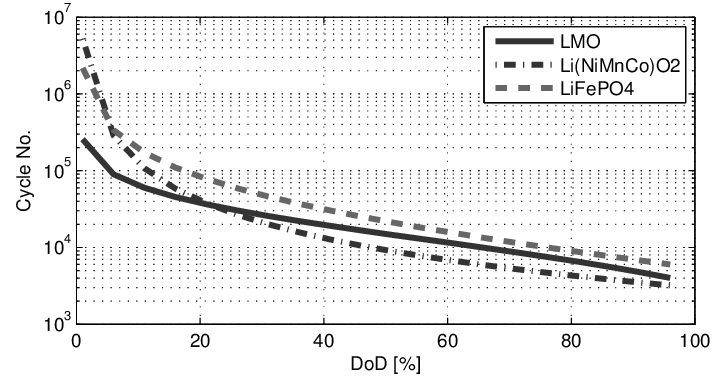
\includegraphics[width=0.45\textwidth]{figures/acc_curves1.png}
        \caption{Typical cycle life of \acp{LIB} as function of \ac{DOD} \cite{XU2016}.}
        \label{fig:acc_curves1}
    \end{figure}

    Note that \ac{DOD} is defined as the positive difference between the initial and final \ac{SOC}, both measured in decimal units, i.e. from 0 to 1. In this formulation it will be represented by $dod$:
%    \begin{equation}
        $$ dod = |s_{0}-s_{f}|$$
%        \label{eq:dod(s)}
%    \end{equation}

    Since life cycle information is usually given at discrete \ac{DOD} levels, it is useful to interpolate those data points. For that, we define a generic function $ACC(dod)$ that may have any format in order to better fit different wear curves.

    The form used for $ACC(dod)$ in \cite{HAN2014} is the reciprocal function: $ACC(dod) = a_{0} \cdot dod^{-a_{1}}$, where $a_{0}$ and $a_{1}$ are coefficients obtained through curve fitting. This provides a good fit for the \ac{ACC} curve of some wear curves but leaves room for improvement into a more universal form.

    Other formats are able to produce good fits, such as the exponential $ACC(dod) = a_0 \mathrm{e}^{-a_1 d}$ and logarithmic $ACC(dod) = a_0 - a_1 \ln(dod)$ forms. Although these elementary functions performed well on specific batteries, they alone fail to provide a universal model. In light of this, the authors propose a combination of the reciprocal and exponential functions:
    \begin{equation}
    	ACC(dod) = a_0 \cdot d^{-a_1} \cdot \mathrm{e}^{-a_2 d}
    	\label{eq:ACC(dod)}
    \end{equation}
    where $a_0$, $a_1$ and $a_2$ are coefficients that can be obtained by methods such as the least squares fitting.

    Equation \eqref{eq:ACC(dod)} proved to be a good empirical model to fit the cycle life curves of different commercial battery chemistries and manufacturers, as shown in Fig. \ref{fig:acc(dod)}. Therefore, this was the format chosen to be implemented in this study.
    \begin{figure}[!h]
    	\begin{subfigure}{.235\textwidth}
    		\centering
    		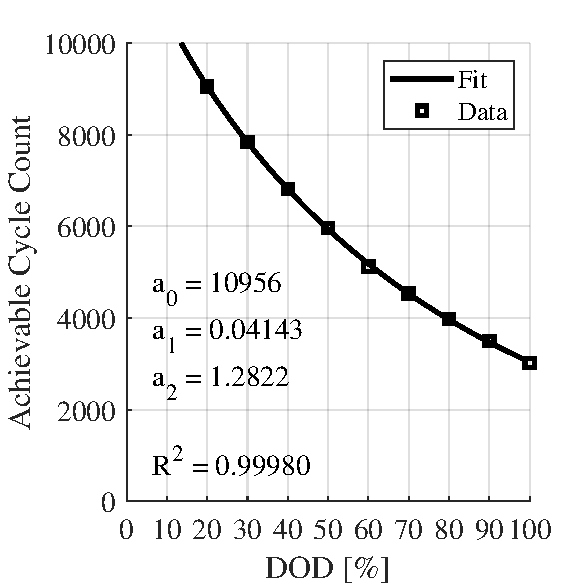
\includegraphics[width=\linewidth]{figures/acc_fitting_NeoVolta_NV24_LiFePO4.pdf}
    		\caption{NeoVolta NV14 (LiFePO4)}
    		\label{fig:accNeovolta}
    	\end{subfigure}
    	\begin{subfigure}{.235\textwidth}
    		\centering
    		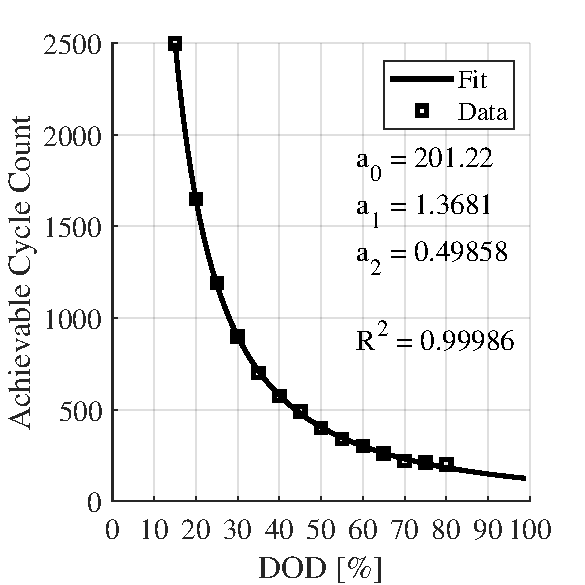
\includegraphics[width=\linewidth]{figures/acc_fitting_Moura_12MF220_lead-acid.pdf}
    		\caption{Moura 12MF220 (lead-acid)}
    		\label{fig:accMoura}
    	\end{subfigure}

    	\begin{subfigure}{.235\textwidth}
    		\centering
    		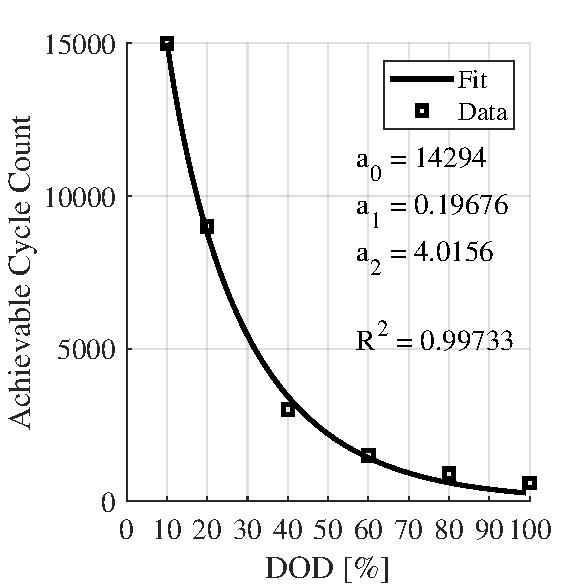
\includegraphics[width=\linewidth]{figures/acc_fitting_Unknown_model_LiPO4.pdf}
    		\caption{Generic model (LiFePO4) \cite{BATUNI2020}}
    		\label{fig:accLipeo4}
    	\end{subfigure}
    	\begin{subfigure}{.235\textwidth}
    		\centering
    		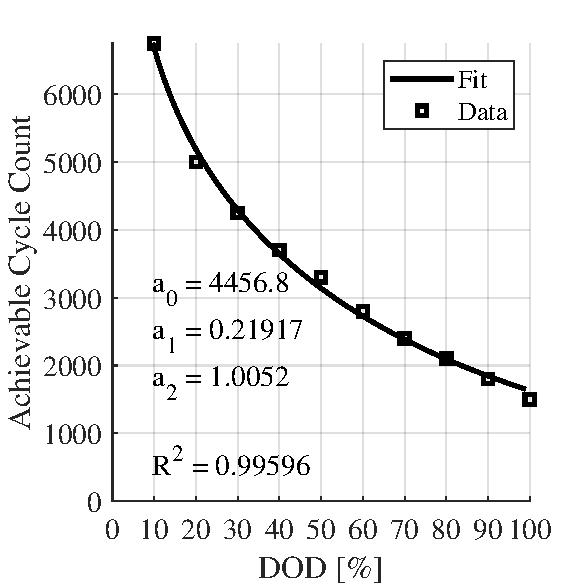
\includegraphics[width=\linewidth]{figures/acc_fitting_Rolls_16CH35P_lead-acid.pdf}
    		\caption{Rolls 8 CH 33P (lead-acid)}
    		\label{fig:accNimh}
    	\end{subfigure}
    	\caption{Equation \eqref{eq:ACC(dod)} fitted to data from different chemistries and manufacturers.}
    	\label{fig:acc(dod)}
    \end{figure}

    \subsection{Cost per cycle --- starting at 100\% SOC}
    Given that $ACC(dod)$, independent of the chosen form, yields the number of times that a battery can be cycled, the ratio between the battery total replacement cost, $B_p$ and $ACC(dod)$ corresponds to the cost of a full cycle of depth $d$:

    $$ \mathrm{Cost \; per \; full \; cycle} = \frac{ \alpha B_p}{ACC(dod)} $$
    Where again, $\alpha$ is a modulating factor to account for temperature fluctuation.

    Then, to assess the cost of a single event (i.e. either the charging or discharging part of a cycle), this value should further be divided by two, thus:
    \begin{equation}
        \mathrm{Cost \; per \; half \; cycle} = \frac{ \alpha B_{P}}{2 \; ACC(dod)}
        \label{eq:costPerHalfCycle1}
    \end{equation}

    That is, if a half cycle either starts or ends at 100\% \ac{SOC}, the \ac{DOD} could be plugged into \eqref{eq:costPerHalfCycle1} and the expression would yield the wear cost associated with that event. As such, by definition, equation \eqref{eq:costPerHalfCycle1} is a solution to the cost function $C_B(s_{0}, s_{f})$ with $s_0 = 1$ for discharing or $s_f = 1$ for charing. However, for ranges that neither start nor end at 100\% \ac{SOC}, a more general expression must be derived.

    \subsection{Cost per cycle --- any range}

    For charging from $s_0$ to 100\%, we replace $dod=|s_{0}-1|$ in \eqref{eq:costPerHalfCycle1} and equate it to \eqref{eq:Cb(s0,sf)}, resulting in:
    \small
%    \begin{equation}
       $$ \int_{s_{0}}^{1}w(s)ds = W(1) - W(s_{0}) = \frac{\alpha B_{P}}{2 \; ACC(|s_{0}-1|)} $$
%        \label{eq:costCharging100}
%    \end{equation}
	\normalsize
    where $W(s)$ is a primitive of $w(s)$ and $s_{0}$ is the lower limit of integration because it will always be less or equal to 1 (there are no \ac{SOC} levels greater than 100\%).

%    Expanding the integral on the left hand side of \eqref{eq:costCharging100}:
%    \begin{equation}
%        W(1) - W(s_{0}) = \frac{\alpha B_{P}}{2 \; ACC(|s_{0}-1|)}
%        \label{eq:fundamentalTheorem1}
%    \end{equation}
%    where $W(s)$ is a primitive of $w(s)$.

    A similar expression can be obtained for a discharging event, when $dod=|1-s_{f}|$, yielding:
    \small
%    \begin{equation}
         $$ \int_{s_{f}}^{1}w(s)ds = W(1) - W(s_{f}) = \frac{\alpha B_{P}}{2 \; ACC(|1-s_{f}|)} $$
%        \label{eq:fundamentalTheorem2}
%    \end{equation}
	\normalsize

    By subtracting the second expression from the first and rewriting in compact integral notation, we arrive at a partial solution to \eqref{eq:Cb(s0,sf)}:
    \small
%    \begin{equation}
       $$ \int_{s_{0}}^{s_{f}}w(s)ds = \frac{\alpha B_{P}}{2 \; ACC(|s_{0}-1|)} - \frac{\alpha B_{P}}{2 \; ACC(|1-s_{f}|)} $$
%        \label{eq:partialSolution}
%    \end{equation}
	\normalsize

    This expression is only positive for $s_{0} \le s_{f}$, that is, for recharging. The process can be repeated for the case where $s_{0} > s_{f}$ and the result would be the same expression with a flipped sign. Instead, a single closed-form equation can be summarized using the modulus operator. The result is the solution to the cost function $C_B(s_{0}, s_{f})$ defined in \eqref{eq:Cb(s0,sf)}:
    \small
    \begin{equation}
        C_B(s_{0}, s_{f}) = \frac{\alpha B_{P}}{2} \left| \frac{1}{ACC(1-s_{f})} - \frac{1}{ACC(1-s_{0})} \right|
        \label{eq:finalSolution}
    \end{equation}
	\normalsize
    where, since both $s_{0}$ and $s_{f}$ are always less or equal to one, the inner modulus operator was discarded.

    The model proposed in \eqref{eq:finalSolution} is valid through the entire \ac{SOC} range, from 0\% to 100\%, as long as $1/ACC(s)$ is continuous in that same range and, since it does not assume any particular format for $ACC(dod)$, it also is fairly independent of battery model.

    This result adds two levels of abstraction to \cite{HAN2014} because it accepts almost any generic form of $ACC(dod)$ without the need to derive a new model. It also uses only the initial and final \ac{SOC} of each half cycle, therefore there's no need to know the power flow of the battery at each instant, only the amount of energy transferred. Again, this is possible due to our initial assumption of moderate C-rates being used in \acp{MG}. This simplification provides a much faster way to calculate costs in a centralized \ac{EMS}, which was the goal set at the beginning of the formulation.

    \subsection{Qualitative Analysis: The Normalized Wear Density Function}
    Although the expression in \eqref{eq:finalSolution} allows an optimization model to quantify the wear of cycling a battery, it fails to provide an easy insight on how cycling the battery at different \ac{SOC} ranges affect its durability. For qualitative analysis, the Wear Cost Density Function, $w(s)$ would provide a better tool to evaluate the performance of a battery.

    For that, we can simply take the partial derivative of the cost function \ref{eq:finalSolution} with respect to $s=s_f$ and divide it by the capacity $M$ of the battery, arriving at a Normalized Wear Density Function $w_n(s)$ in terms of monetary unit per unit of energy transferred (usually \$/kWh):
    \small
%    \begin{equation}
		$$ w_n(s) = \frac{w(s)}{M} = \frac{\partial}{\partial s} \frac{- \alpha B_P}{2 \cdot M \cdot ACC(1-s)} $$
%        \label{eq:wn(s)}
%    \end{equation}
	\normalsize

    By substituting \eqref{eq:ACC(dod)} into it and considering $ s \le 1 $, the normalized Wear Density Function becomes:
    \small
    \begin{equation}
        w_n(s) = \frac{\alpha B_P}{2M} \cdot \frac{a_1(1-s)^{a_1-1} + a_2(1-s)^{a_1}}{a_0} \cdot \mathrm{e}^{a_2(1-s)}
        \label{eq:wn(s)a0a1a2}
    \end{equation}
	\normalsize

	This function is able to show where in the \ac{SOC} range the most wear occur. Moreover, the average value of the Wear Density Function is also useful when evaluating the overall cost-benefit of different battery models, as it can differentiate batteries not only by price and capacity, but also by durability. The average value of \eqref{eq:wn(s)a0a1a2} is calculated as:
%    \begin{equation}
		$$ \overline{w_n} = \frac{\alpha B_P}{2M} \frac{\mathrm{e}^{a_2}}{a_0} $$
%    \end{equation}
	which could also be a useful expression for a linear cost function, such as $C_B(s_0, s_f) = \overline{w_n}  \cdot M \cdot |s_f - s_0|$.

    \section{Energy Management Model}
    To test the battery wear model, we modified the optimization problem proposed by \cite{SANTOS2018}, which initially used a fixed cost per kilowatt-hour to evaluate the cost of using the \ac{BESS}. The model implements a day-ahead planning strategy using \ac{MILP} that aims to minimize the operational cost of \iac{MG} composed by a \ac{DG}, \iac{BESS}, \iac{PV} system and a load, as illustrated by Fig. \ref{fig:mg1}.
    \begin{figure}[htbp]
        \centering
        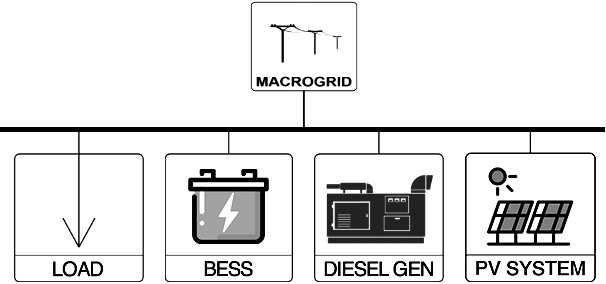
\includegraphics[width=0.4\textwidth]{figures/mg2.png}
        \caption{Diagram of the simulated \ac{MG}.}
        \label{fig:mg1}
    \end{figure}

    The objective of the optimizer is to calculate setpoints that all DERs within the \ac{MG} should follow in order to supply demand with the lowest operational cost. This may lead to strategies such as charging batteries in off-peak hours to minimize energy purchase during peak-hours, therefore the importance of having a model to quantify battery wear in the same manner that other sources have, such as fuel cost for \acp{DG} or energy purchase cost from utility grid.

    The \ac{MG} is modeled as a single-bus system and, as such, no distribution line losses are considered. The model also does not account for the dynamic behavior of the DERs, as this is an attribution of local controllers. The day-ahead planning is based on predictions of load profiles and solar generation profiles for the following 24 hours, this predictions can be obtained from external APIs that are not the focus of this work.

    Two electricity tariff levels are considered, one for peak and one for off-peak hours, and also two contracted demand levels for those periods. Reverse power-flow is rewarded with a feed-in tariff that is a fraction of the energy purchase tariff.

    The model uses a discrete-time approach with finer timesteps for the first hour and larger timesteps for the remaining 23 hours. The first half hour is quantized in 6 intervals of 5 minutes each; then there is a single 30 minute interval followed by 23 intervals of 60 minutes each. This ensures higher time-definition for the near-future while also minimizing the amount of equations of the resulting model. This is important for a centralized model in which forecasts are updated and setpoints recalculated every few minutes, a scenario that can be challeging to sustain in a system with a large number of \acp{MG}.

    \subsection{Objective Function}
    \label{subsec:obj_func}
    The objective function that defines the optimization problem of this study is the sum of operational costs and energy purchase expenses at each discretization interval:
    \begin{equation}
        Z = \sum_{t=1}^T(Z_{IO}[t] + Z_D[t] + Z_B[t] + Z_P[t])
        \label{eq:z1}
    \end{equation}
    where:
    \begin{itemize}
        \item $Z$: total operational cost over the simulation period;
        \item $t$: time-discretization index (1, 2, 3...);
        \item $T$: discretization interval count;
        \item $Z_{IO}$: energy import cost ($+$) or export revenue ($-$);
        \item $Z_{D}$: operational cost of the \ac{DG};
        \item $Z_{B}$: battery wear cost; and
        \item $Z_{P}$: penalty for exceeding maximum contracted demand.
    \end{itemize}

    Notice that there is no term associated with \ac{PV} system power output because its operational cost is usually independent of energy delivery.

    \textbf{Energy import cost and export revenue} --- modeled with a feed-in tariff:
    \begin{equation}
        Z_{IO}[t] = \left( \mu_i[t] \cdot P_i[t] - \mu_e[t] \cdot P_e[t] \right) \cdot dt[t]
    \end{equation}
    where $\mu_i[t]$ and $\mu_e[t]$ are the purchase and feed-in tariffs parameters, respectively; $P_{i}[t]$ and $P_{e}[t]$ are the power import and export variables, respectively; and $dt[t]$ is the size of the discretization interval parameter. Note that power imported at a rate under the contracted limit is calculated separately from the power imported above the contracted limit, that is, $P_i[t]$ is always lower then the contracted demand.

    \textbf{Diesel fuel cost} --- the cost of diesel fuel, modeled using a quadratic model and a startup cost:
    \begin{equation}
        Z_D[t] = \mu_d \cdot (a^{}_d P_d[t]^{2} + b_dP_d[t] + c_d) \cdot dt[t] + S_d[t]
    \end{equation}
    where $\mu_d$ is the cost per liter of diesel; $a_d$, $b_d$ and $c_d$ are the consumption parameters of the \ac{DG}; $P_d[t]$ is the power output variable of the \ac{DG}; and $S_d[t]$ is the startup cost variable of the generator at each discretization interval, which is zero if the generator has been started at a previous interval or if the power output is zero. The power output of the \ac{DG} is also subject to minimum and maximum limits.

    \textbf{Maximum demand penalty} --- modeled using a very high tariff for power import:
    \begin{equation}
        Z_P[t] = \mu_{pi}[t] \cdot P_{pi}[t] \cdot dt[t]
    \end{equation}
    where $\mu_{pi}[t]$ is the parameter that defines the tariff for buying power at a rate above the contracted limit, usually several times higher then $\mu_i[t]$; and $P_{pi}[t]$ is the variable for importing power above the contracted limit, which is only greater then zero when $P_i[t]$ has reached the contracted demand limit.

    \textbf{Battery wear cost} --- obtained by substituting \eqref{eq:ACC(dod)} in \eqref{eq:finalSolution}, where the initial and final \ac{SOC}, $s_0$ and $s_f$, become $s[t-1]$ and $s[t]$, respectively:
    \small
    \begin{equation}
        \begin{aligned}
            C_B[t] & = \frac{B_P}{2a_0} \Bigg|(1-s[t])^{a_1}\mathrm{e}^{a_2(1-s[t])} \\
            & - (1-s[t-1])^{a_1}\mathrm{e}^{a_2(1-s[t-1])} \Bigg|
        \end{aligned}
    	\label{eq:cb[t]_implemented}
    \end{equation}
	\normalsize
	this model is then linearized using a technique of Piecewise-Linear Approximations of Multidimensional Functions before insertion into the \ac{MILP} problem.

    In order to realize the power balance of the \ac{MG}, the power output of the battery is calculated by converting battery percentage to energy transfer rate, i.e. $P_b[t] = \frac{M(s[t]-s[t-1])}{dt[t]}$, which is negative for battery recharge.

    The mathematical modeling is described in detail \cite{SANTOS2018}, with the clear exception of the current battery wear model. For briefness, this work will continue to focus on the battery modeling and the interested reader can refer to the original paper for a detailed explanation of the entire model.

    \section{Methodology \& Simulations}
    \subsection{Software assistant}
    To validate the proposed battery model, we tested it under various scenarios, with different \ac{MG} topology, battery models and load profiles. To assist in this process, a software was developed, as illustrated by Figs. \ref{fig:adams1} and \ref{fig:adams2}.
    \begin{figure}[!h]
    	\centering
    	\begin{subfigure}{0.45\textwidth}
    		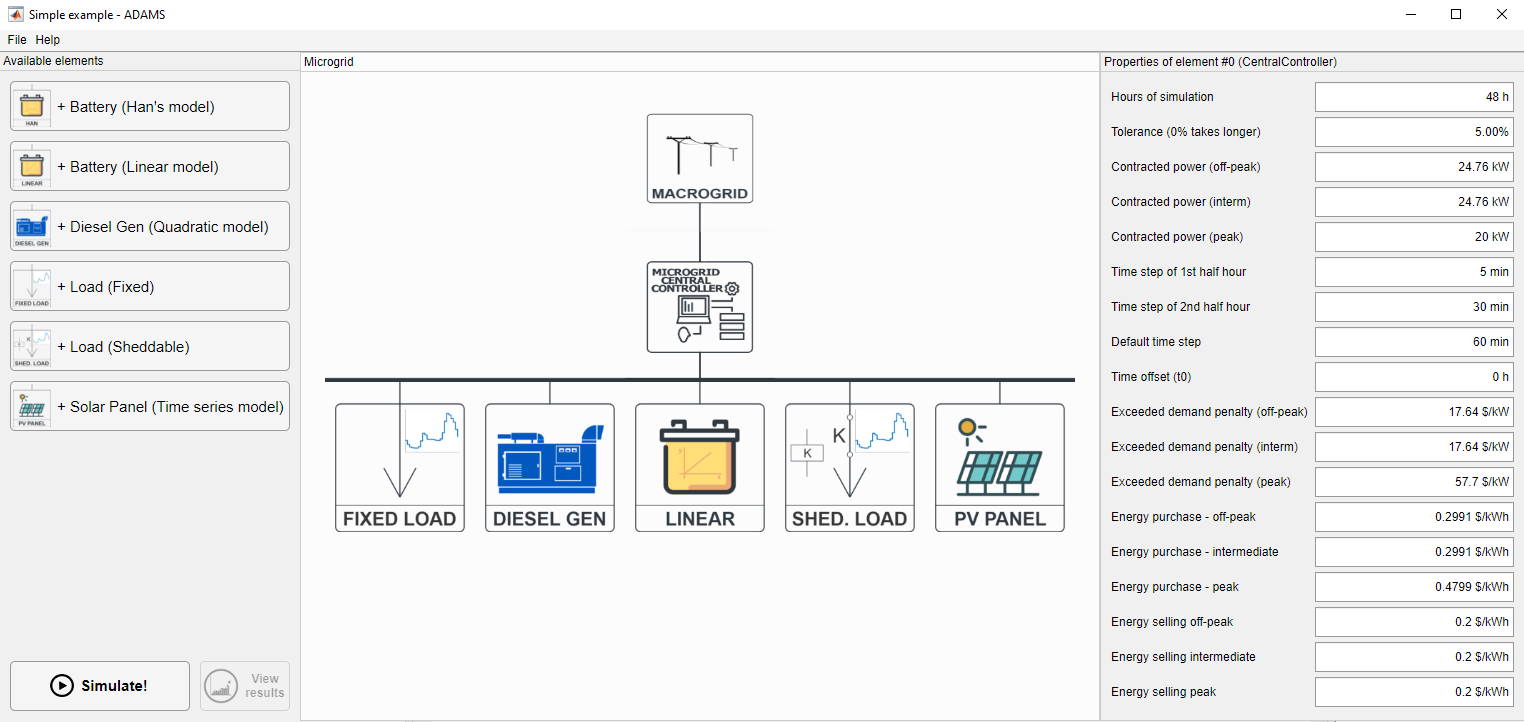
\includegraphics[width=\linewidth]{figures/ss1.png}
    		\caption{Scenario configuration}
    		\label{fig:adams1}
    	\end{subfigure}

    	\begin{subfigure}{0.45\textwidth}
    		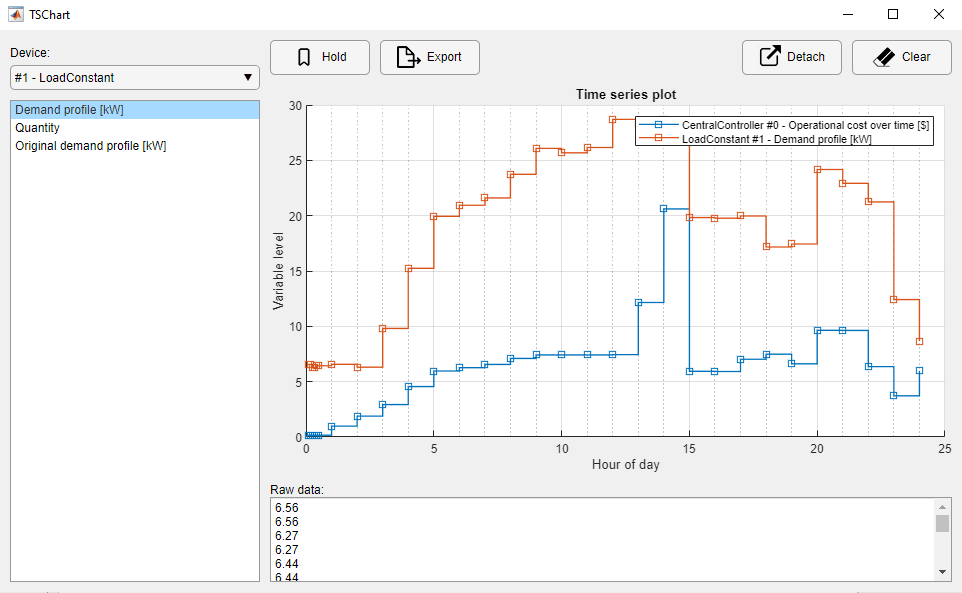
\includegraphics[width=\linewidth]{figures/ss2.png}
    		\caption{Simulation results}
    		\label{fig:adams2}
    	\end{subfigure}
    \end{figure}
	After the user selects which resources the \ac{MG} will contain, the application dynamically generates and solves the optimization problem as described in subsection \ref{subsec:obj_func}. The underlying mathematical model is generated using \ac{MILP} and the user has the option to export the generated code if they want to fine-tune parameters and the behavior of the simulation. The software also also includes an islanded operation mode which is not part of this particular study, but can be useful to test critical scenarios where storing energy is essential. It is free to use and open sourced, available at \href{https://github.com/lucasrhode95/adams}{github.com/lucasrhode95/adams}. All the results presented in this paper were generated using this tool.

    \subsection{Component parameters selection}
    Parameters for the simulations were based on commercially available products with public data made available by the manufacturer of each product.

    \textbf{Energy Sources} -- the \ac{DG} parameters are from a Caterpillar's DE22E3 22 kVA module and the \ac{PV} generation is from a generic autumn profile scaled to deliver 100 kWh/day.

    As for the utility grid, the average electricity rates in Brazil were used: off-peak prices were set at 0.1048 USD/kWh and peak prices at 0.2096 USD/kWh. Feed-in tariff was set at 0.035 USD/kWh for peak and off-peak hours. The contracted demand at was defined as 23 kW and 18.4 kW for off-peak and peak-hours, respectively. Above these limits, tariffs were defined as 10 USD/kWh for off-peak hours and 20 USD/kWh for peak-hours.

    \textbf{Load} -- the residential load profile used was obtained from the U.S. Department of Energy public database \cite{DOE2013} and scaled to achieve a consumption of 300 kWh/day.

    The net load profile (load consumption minus \ac{PV} generation) is shown in Fig. \ref{fig:net-load}, where it can be seen that the \ac{PV} generation exceeds demand from 10 a.m. to 14 a.m., where the "net load" curve becomes negative. In this window it is expected that the \ac{EMS} either chooses to recharge the battery or to export power back into the grid.
    \begin{figure}[htbp]
        \centering
        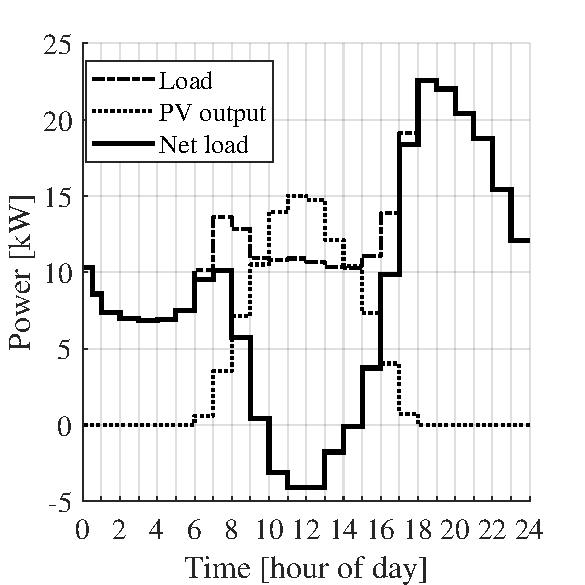
\includegraphics[width=0.3\textwidth]{figures/net_load.pdf}
        \caption{Profiles for residential load, \ac{PV} generation and the resulting net load used.}
        \label{fig:net-load}
    \end{figure}

	\textbf{Storage} -- two \ac{BESS} models were considered, with data acquired directly from the manufacturer's website: NeoVolta's NV14 (14.4 kWh) and Rolls' 8 CH 33P (7.12 kWh), referred as \ac{BESS} A and \ac{BESS} B, respectively. The cycle-life curve, $ACC(dod)$, of each system was extracted directly from their datasheet and are presented in Fig. \ref{fig:acc(dod)2}. The data points where extracted by superimposing points over the graphic, relating the graphical coordinates with the indicated axes and performing a curve-fitting. The format used is as proposed in eq. \ref{eq:ACC(dod)}.
	\begin{figure}[!h]
		\begin{subfigure}{.235\textwidth}
			\centering
			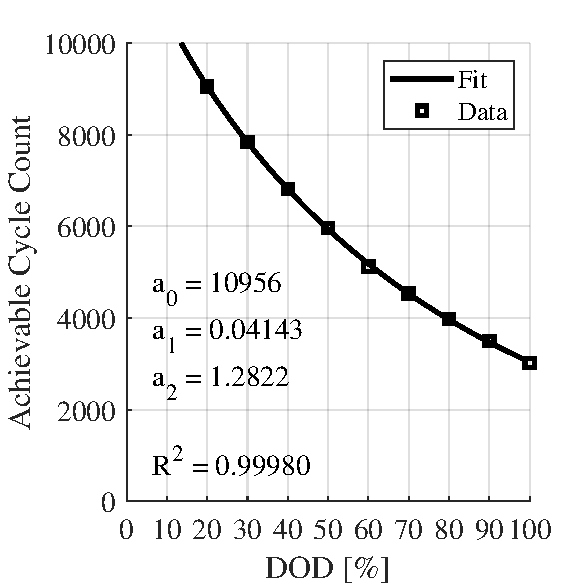
\includegraphics[width=\linewidth]{figures/acc_fitting_NeoVolta_NV24_LiFePO4.pdf}
			\caption{BATTERY A (LiFePO4)}
			%    		\caption{NeoVolta NV14 (LiFePO4)}
			\label{fig:accNeovolta2}
		\end{subfigure}
		\begin{subfigure}{.235\textwidth}
			\centering
			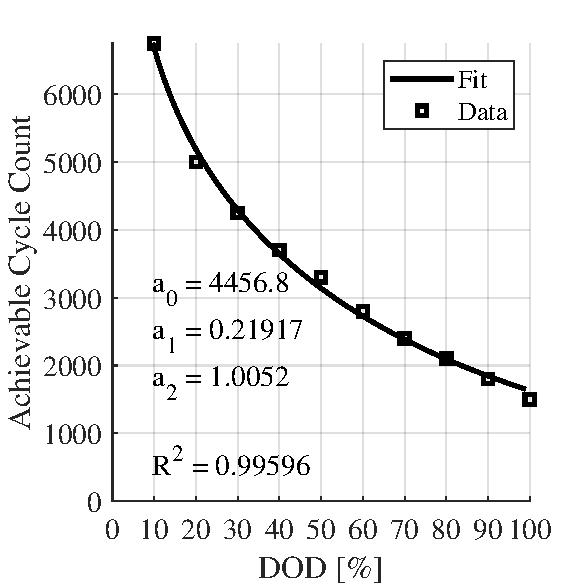
\includegraphics[width=\linewidth]{figures/acc_fitting_Rolls_16CH35P_lead-acid.pdf}
			\caption{BATTERY B (lead-acid)}
			%    		\caption{Rolls 8 CH 33P (lead-acid)}
			\label{fig:accNimh2}
		\end{subfigure}
		\caption{Equation \eqref{eq:ACC(dod)} fitted to data from different chemistries and manufacturers.}
		\label{fig:acc(dod)2}
	\end{figure}

    The wear density of both is shown in Fig. \ref{fig:wn_curves1}, where the lowest wear density points are highlighted: 0.088123 USD/kWh at 87\% \ac{SOC} for \ac{BESS} A, and 0.18287 USD/kWh at 75\% \ac{SOC} for \ac{BESS} B. It also can be observed that wear density increases at both ends of the \ac{SOC}, an expected result given that both very low and very high \ac{SOC} levels are known to reduce battery life \cite{ECKER2014, WIKNER2018}.
    \begin{figure}[!h]
        \begin{subfigure}{.235\textwidth}
            \centering
            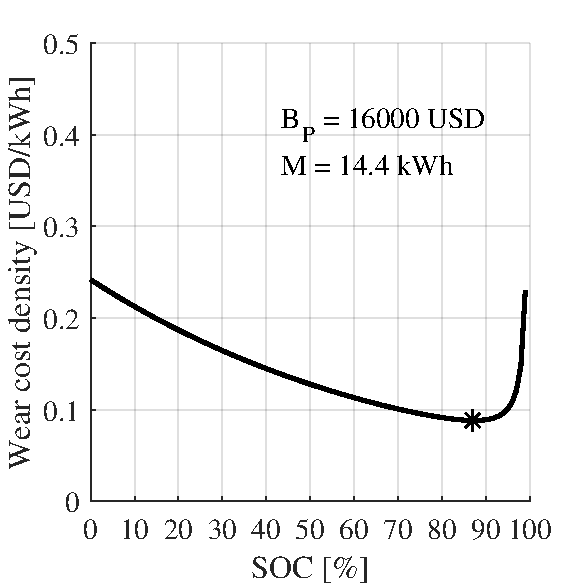
\includegraphics[width=\linewidth]{figures/marginal_NeoVolta_NV24_LiFePO4.pdf}
            \caption{\ac{BESS} A (LiFePO4)}
            \label{fig:wn_curves1A}
        \end{subfigure}
        \begin{subfigure}{.235\textwidth}
            \centering
            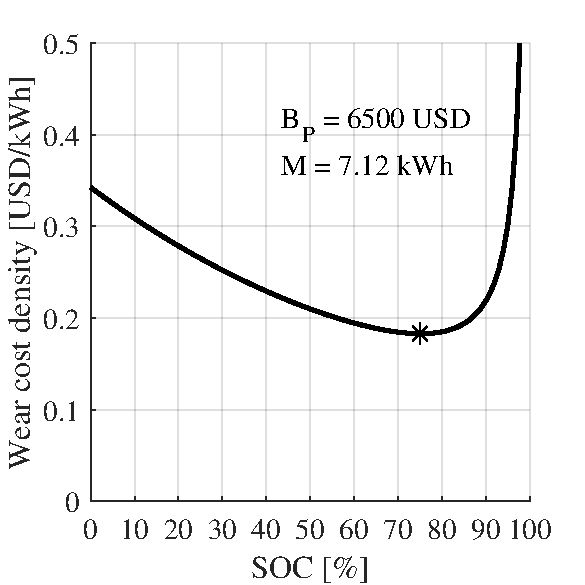
\includegraphics[width=\linewidth]{figures/marginal_Rolls_8CH33P_lead-acid.pdf}
            \caption{\ac{BESS} B (lead-acid)}
            \label{fig:wn_curves1B}
        \end{subfigure}
        \caption{Wear Density Function of both batteries.}
        \label{fig:wn_curves1}
    \end{figure}

    For the tests, both systems were considered to have an efficiency of 94\% (yielding a round-trip efficiency of 88.36\%), a self discharge rate of 0.2\% per hour and charge/discharge rate was limited to 0.5C. In order to keep both systems with roughly the same capacity, we considered that \ac{BESS} B is composed of two batteries, therefore doubling its cost and capacity to 13,000 USD and 14.24 kWh, respectively. In addition, the \ac{SOC} of both systems were arbitrarily set to start at 50\%.

    Another restriction is that battery must also have 50\% \ac{SOC} at the end of the day so that all energy usage must be replenished before the end of the simulation, plus losses.

    \subsection{Results}
    The results were collected from a simulation with a 24-hour horizon, with initial \ac{SOC} (i.e. when $t=0$) equal to 50\%. The \ac{DG} starts offline with a power dispatch of 0 kW. The \ac{PV} source output and load profile are as shown in \ref{fig:adams2}. These curves and initial conditions are inserted into the \ac{MILP} model and runned as to minimize the objective function (see eq. \ref{fig:mg1}).

    There were four scenarios analyzed with varying composition of \ac{BESS} models and \ac{DG} availability, always under the same net load presented in Fig. \ref{fig:net-load}. The scenarios analyzed and their respective operational cost for a simulated 24-hour operation were:
    \begin{enumerate}
        \item \label{item:bessa+diesel} \textbf{Scenario \ref{item:bessa+diesel}:} \ac{BESS} A + \ac{DG}, 29.7763 USD;
        \item \label{item:bessb+diesel} \textbf{Scenario \ref{item:bessb+diesel}:} \ac{BESS} B + \ac{DG}, 30.7006 USD;
        \item \label{item:bessb} \textbf{Scenario \ref{item:bessb}:} \ac{BESS} B only, 31.7940 USD;
        \item \label{item:diesel} \textbf{Scenario \ref{item:diesel}:} \ac{DG} only, 30.6420 USD.
    \end{enumerate}

    Considering an error tolerance of 1\%, scenarios \ref{item:bessb+diesel} and \ref{item:diesel} are equivalent in regard of operational cost. That is, the addition of \ac{BESS} B to a system where there is already a \ac{DG} produces no substantial benefit from the energy management perspective alone. However, there are indubitably many advantages of having both systems at disposal and, as such, this result should not be taken as definitive for all cases.

    The detailed results of the day-ahead planning for scenarios \ref{item:bessa+diesel} and \ref{item:bessb+diesel} are shown in Fig. \ref{fig:results}, with the following highlights:
    \begin{figure}[!h]
        \begin{subfigure}{.235\textwidth}
            \centering
            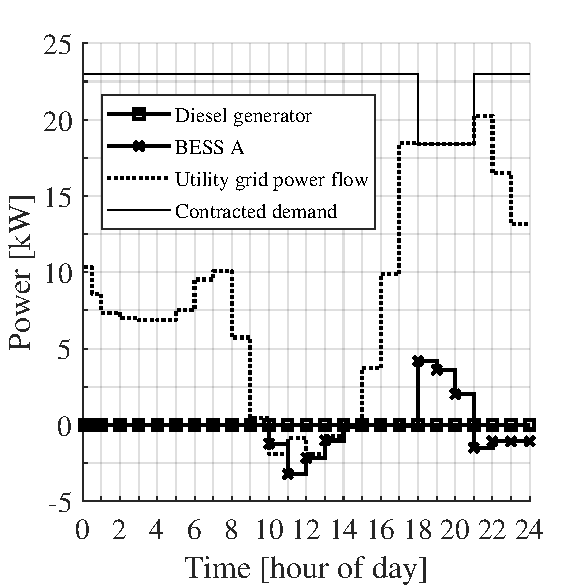
\includegraphics[width=\linewidth]{figures/residential_nv14_power.pdf}
            \caption{Power curves for scenario \ref{item:bessa+diesel}}
            \label{fig:result-power-A}
        \end{subfigure}
        \begin{subfigure}{.235\textwidth}
            \centering
            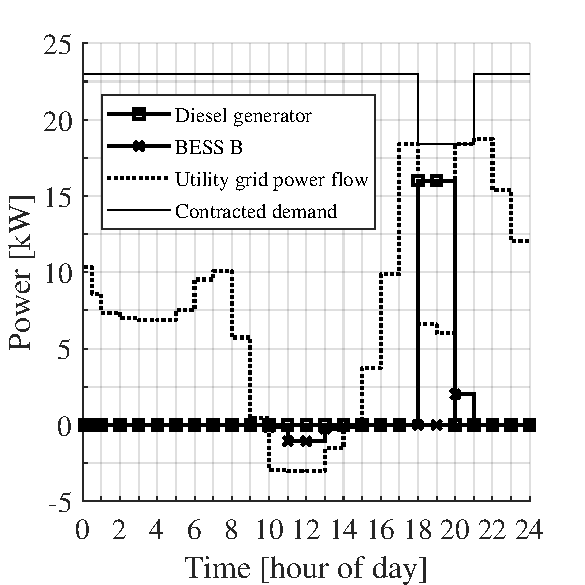
\includegraphics[width=\linewidth]{figures/residential_8ch33p_power.pdf}
            \caption{Power curves for scenario \ref{item:bessb+diesel} }
            \label{fig:result-power-B}
        \end{subfigure}

        \begin{subfigure}{.235\textwidth}
            \centering
            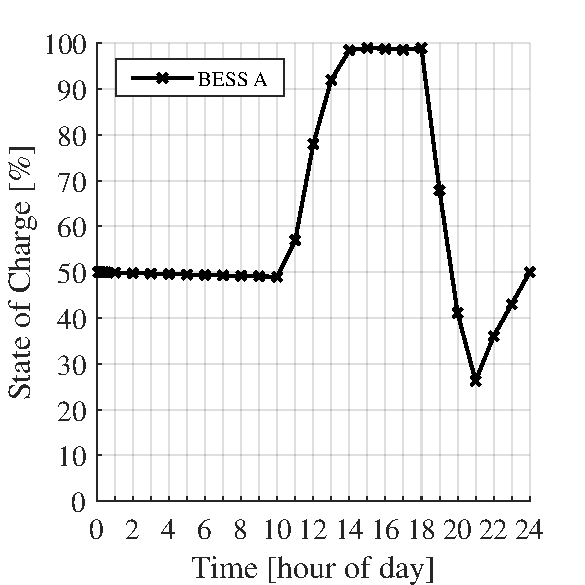
\includegraphics[width=\linewidth]{figures/residential_nv14_soc.pdf}
            \caption{Battery's \ac{SOC} for scenario \ref{item:bessa+diesel}}
            \label{fig:result-soc-A}
        \end{subfigure}
        \begin{subfigure}{.235\textwidth}
            \centering
            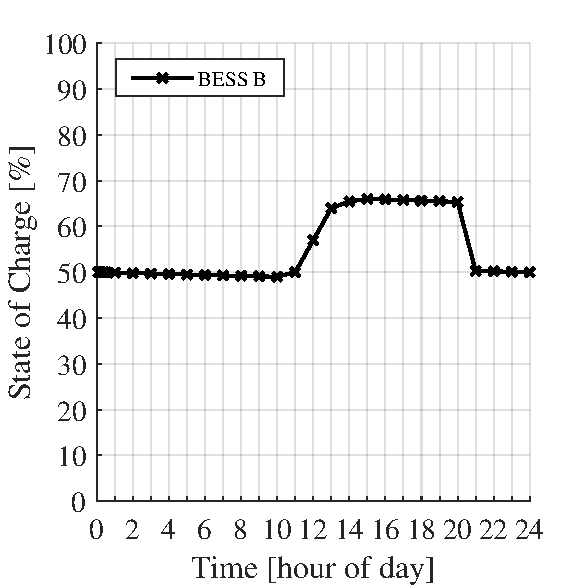
\includegraphics[width=\linewidth]{figures/residential_8ch33p_soc.pdf}
            \caption{Battery's \ac{SOC} for scenario \ref{item:bessb+diesel}}
            \label{fig:result-soc-B}
        \end{subfigure}
        \caption{Results of the day-ahead planning for each battery system.}
        \label{fig:results}
    \end{figure}

    \begin{itemize}
        \item \textbf{0 a.m. -- 6 a.m.:} no \ac{PV} generation, load is supplied only by the grid while, in both cases, neither \ac{BESS} nor \ac{DG} is active. Batteries self discharge at a 0.2\% rate;
        \item \textbf{6 a.m. -- 10 a.m.:} \ac{PV} generation gradually increases, until net load drops to zero;
        \item \textbf{10 a.m. -- 3 p.m.:} \ac{PV} generation continues to increase, surpassing demand. Excess generation is used to charge batteries from 49.0\% to 99.0\% in scenario \ref{item:bessa+diesel} and to 66.0\% in scenario \ref{item:bessb+diesel};
        \item \textbf{3 p.m. -- 6 p.m.:} \ac{PV} generation gradually decreases until zero. Batteries are kept in stand-by;
        \item \textbf{6 p.m. -- 9 p.m.:} to avoid excess demand and subsequent penalties, \ac{BESS} A is cycled from 99.0\% to 26.2\% to diminish energy purchase in scenario \ref{item:bessa+diesel}, supplying roughly 10.5 kWh to the system. In contrast, in scenario \ref{item:bessb+diesel}, the \ac{DG} is started at 6 p.m. and stopped at 8 p.m., delivering exactly 32 kWh in two hours. This power output is more than enough to avoid excess demand and also to minimize peak-hour energy purchase --- until the quadratic consumption model limits its benefits. In the following hour, from 8 p.m. until 9 p.m., \ac{BESS} B is cycled from 65.4\% to 50.3\% to supply the system.
        \item \textbf{9 p.m. -- 12 p.m.} the load curve starts to fade to a minimum whilst \ac{BESS} A is recharged in scenario \ref{item:bessa+diesel} and \ac{BESS} B is kept in stand-by until midnight on \ref{item:bessb+diesel}.
    \end{itemize}

    The main difference between scenarios \ref{item:bessa+diesel} and \ref{item:bessb+diesel} is notably the much deeper \ac{DOD} cycle that \ac{BESS} A experiences. This is due to the lower marginal cost when compared to \ac{BESS} B, as can be seen in Fig. \ref{fig:wn_curves1}.

    Another interesting result is the choice of \ac{SOC} range that the optimizer made for \ac{BESS} A. The 10.5 kWh that it delivered represents 73\% of its capacity, and could have been cycled in either 100\%-27\% or 73\%-0\% ranges, for example. However, the 99\%-26\% indicates that the optimizer avoided the steep wear density rise near 100\% but also tried to avoid the slowly increasing wear cost near the lower end of the \ac{SOC}. The same trend is observed in scenario \ref{item:bessb+diesel} but, with a much more steep rise near 100\% and overall higher wear cost, the battery is only cycled with a \ac{DOD} little greater than 16\%.

    In summary, this results demonstrate that the model induces the optimizer, and therefore the management system, to cycle the battery at \ac{SOC} ranges that minimize wear, without blocking the \ac{BESS} from being used. We specifically mention this since in some configurations the optimizer could choose not to use the batteries at all, specially if \ac{DG}'s startup and fuel costs are very low.

    \section{Conclusion}
    Although battery wear is sometimes neglected in \ac{MG} applications, it is important to incorporate a wear quantification model to avoid careless use of the storage system. In this study we expanded the reach of an existing model by re-deriving it using a more universal approach for fitting the data usually made available by manufacturers. We also provided a mathematical formula that enables \ac{MG} planners to evaluate and compare batteries across the entire \ac{SOC} range, taking into account not only price and capacity, but also the durability of storage devices, and that could be easily customized for various batteries. The model, although simple, proved to be very useful in the implementation of an energy management algorithm that considers and minimizes battery wear, as shown by the case studies presented here, which can effectively prolong the lifespan of these devices.

    \bibliographystyle{./IEEEtran}
    \bibliography{./bibliography}

\EOD
\end{document}
